\documentclass[11pt]{article}
\usepackage[spanish]{babel}
\usepackage{amsmath}  % Math
\usepackage{amssymb}  % Symbols
\usepackage{graphicx} % Images
\graphicspath{ {./images/} }
\usepackage[utf8]{inputenc}
\usepackage[T1]{fontenc}
\usepackage[margin=1in]{geometry}
\usepackage{fancyhdr} % Para el pie de página personalizado
\usepackage{hyperref} % Para metadatos y enlaces en el PDF
\usepackage{listings}
\usepackage{xcolor} % Para definir y usar colores

% ----- CONFIGURACIÓN DE AUTORÍA Y PIE DE PÁGINA -----
\hypersetup{
    pdftitle={Tu Título},
    pdfauthor={Felipe Colli Olea},
    colorlinks=true,
    linkcolor=black,
    urlcolor=cyan
}

\lstset{
  language=C++, % Specify the programming language
  numbers=left,      % Add line numbers on the left
  numberstyle=\tiny\color{gray}, % Style for line numbers
  basicstyle=\ttfamily, % Basic font style for code
  keywordstyle=\color{blue}, % Style for keywords
  commentstyle=\color{green}, % Style for comments
  stringstyle=\color{red},   % Style for strings
  showstringspaces=false, % Do not show spaces within strings
  breaklines=true, % Allow lines to break
  frame=single, % Add a frame around the code block
}


% Configuración del pie de página con fancyhdr
\pagestyle{fancy}
\fancyhf{} % Limpia la cabecera y el pie de página actuales
\fancyfoot[C]{\footnotesize Felipe Colli, Todos los Derechos Reservados} % Tu texto en el centro
\fancyfoot[R]{\thepage} % Número de página a la derecha
\renewcommand{\headrulewidth}{0pt} % Elimina la línea de la cabecera

\title{Apunte Arduino UGM}
\author{Felipe Colli Olea}
\date{\today}

\begin{document}

\maketitle
\thispagestyle{fancy} % Aplica el estilo de pie de página a la primera página también

\newpage
\tableofcontents
\newpage

\section{Prender Leds}
\begin{lstlisting}[caption=Prender leds basicos]
// C++ code
//
int p = 13;
int p2 = 12;

void setup(){
  pinMode(p, OUTPUT);
  pinMode(p2, OUTPUT);
}

void loop() {
  digitalWrite(p2, LOW);
  digitalWrite(p, HIGH);
  delay(500); // Wait for 1000 millisecond(s)
  digitalWrite(p2, HIGH);
  digitalWrite(p, LOW);
  delay(500); // Wait for 1000 millisecond(s)
}

\end{lstlisting}

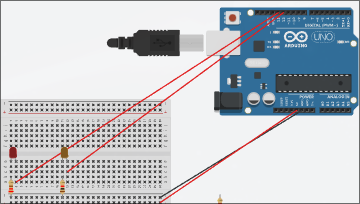
\includegraphics[width=0.5\textwidth]{LEDS}


\end{document}
